\documentclass[11pt, oneside]{article} 
\usepackage{geometry}
\geometry{letterpaper} 
\usepackage{graphicx}
	
\usepackage{amssymb}
\usepackage{amsmath}
\usepackage{parskip}
\usepackage{color}
\usepackage{hyperref}

\graphicspath{{/Users/telliott_admin/Tex/png/}}
% \begin{center} 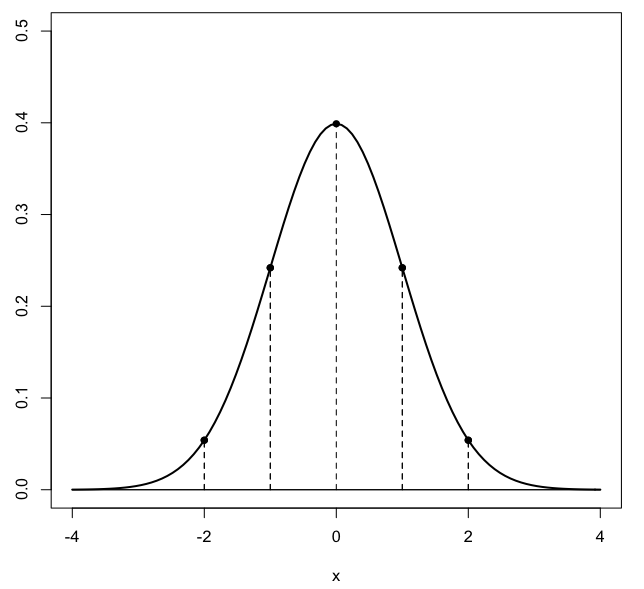
\includegraphics [scale=0.4] {gauss3.png} \end{center}

\title{Vectors to solve the headlight problem}
\date{}

\begin{document}
\maketitle
\Large

\begin{center} 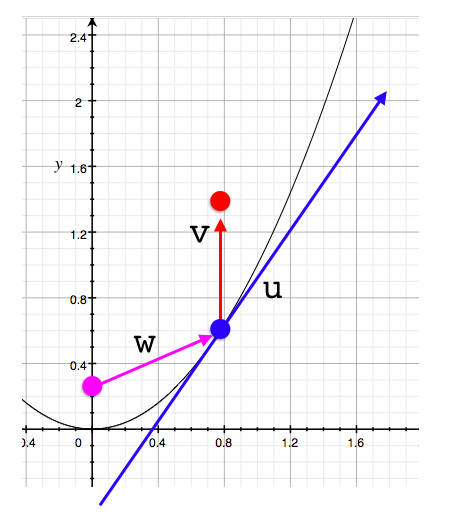
\includegraphics [scale=0.5] {headlight.png} \end{center}

The parabola has the property that every ray of light parallel to the $y$-axis will bounce off the curve and go to the same point, which is called the \emph{focus} of the parabola.  We will prove this here using vectors, making use of the property from optics that a reflected ray makes equal angles of incidence and reflection.

We pick an arbitrary point on the parabola $P = (x,ax^2)$, shown in blue, and draw the tangent to the curve at that point.  The slope of the tangent is $2ax$.  The point $Q = (0,p)$, in magenta, is the focus.

Consider three vectors, one of each color.  The one in blue is 
\[ \mathbf{u} = \langle 1, 2ax \rangle \]
The one in red is
\[ \mathbf{v} = \langle 0, 1 \rangle \]
And the one in magenta is 
\[ \mathbf{w} = \langle x, ax^2 - p \rangle \]
Hopefully, you can derive these yourself.

\subsection*{setup}
The key fact we use is the property from optics, which says that the angle between the blue and red vectors (let's call it $\theta$) is equal to that between the magenta and blue vectors ($\phi$).  If that is true, then their cosines are also equal.  Thus we can write:
\[ \cos \theta = \cos \phi \]
But by the definition of the dot product:
\[ \cos \theta = \frac{ \mathbf{u} \cdot \mathbf{v} }{ |\mathbf{u}| |\mathbf{v}|}
\]
\[ \cos \phi = \frac{ \mathbf{w} \cdot \mathbf{u} }{ |\mathbf{w}| |\mathbf{u}|}
\]
Substituting into first equality, we  write
\[ \frac{ \mathbf{u} \cdot \mathbf{v} }{ |\mathbf{u}| |\mathbf{v}|}
 = \frac{ \mathbf{w} \cdot \mathbf{u} }{ |\mathbf{w}| |\mathbf{u}|} \]
\[ \frac{ \mathbf{u} \cdot \mathbf{v} }{ |\mathbf{v}|}
 = \frac{ \mathbf{w} \cdot \mathbf{u} }{ |\mathbf{w}|} \]

\subsection*{calculation}
What remains is just arithmetic.
\[  \mathbf{u} \cdot \mathbf{v} = \langle 1, 2ax \rangle \cdot \langle 0, 1 \rangle = 2ax \]
\[  \mathbf{w} \cdot \mathbf{u} = \langle x, ax^2 - p \rangle \cdot \langle 1, 2ax \rangle = x + 2ax(ax^2 - p) \]
To make things a bit simpler, define $h = ax^2 - p$.  Then
\[  \mathbf{w} \cdot \mathbf{u} = \langle x, h \rangle \cdot \langle 1, 2ax \rangle = x + 2axh \]

Substitute for the dot products
\[ \frac{ 2ax}{ |\mathbf{v}|}
 = \frac{x + 2axh}{ |\mathbf{w}|} \]
 
We chose $| \mathbf{v} | = 1$ and $| \mathbf{w} | = \sqrt{x^2 + (ax^2 - p)^2} = \sqrt{x^2 + h^2}$.  Substituting for $|\mathbf{w}|$ we obtain:
\[ 2ax = \frac{x + 2axh}{\sqrt{x^2 + h^2}} \]
\[ 2ax \sqrt{x^2 + h^2} = x + 2axh \]
Divide by $x$
\[ 2a \sqrt{x^2 + h^2} = 1 + 2ah \]

Square both sides:
\[ 4a^2 \ [ \ x^2 + h^2 \ ] = 1 + 4ah + 4a^2h^2 \]
\[ 4a^2x^2 + 4a^2h^2 = 1 + 4ah + 4a^2h^2 \]
\[ 4a^2x^2 = 1 + 4ah \]

Reverse the substitution
\[ 4a^2x^2 = 1 + 4a(ax^2 - p) = 1 + 4a^2x^2 - 4ap \]
 We obtain:
\[ 0 = 1 - 4ap \]
\[ 4ap = 1 \]
\[ p = \frac{1}{4a} \]
This is indeed the definition of the focal point.  Furthermore, $p$ is not dependent on $x$, so we obtain the desired result:  every perpendicular ray ends up at the focus.  Conversely, in the case of a headlight, every ray emitted at the focus ends up exiting vertically upwards.


\end{document}